\chapter[Resultados Parciais]{Resultados Parciais}
\label{sec:resultados_parciais}

Com a conclusão da primeira etapa da pesquisa, algumas informações referentes a situação atual do projeto podem ser apresentadas. Com este objetivo, este capítulo se sub-divide nas seções de \textit{Revisão Sistemática}, \textit{Desenvolvimento prático} e \textit{Ações futuras}.

\section{Revisão Sistemática} % (fold)
\label{sec:revisão_sistemática}

	Com o objetivo de detalhar a revisão sistemática realizada durante esse trabalho de forma clara e objetiva, esta seção está divida nas seções de \ref{sub:planejamentoRevisao}, \ref{sub:conducaoRevisao} e \ref{sub:publicacaoRevisao}, seguindo o conceito apresentado por \cite{Kitchenham}, como mostra a figura \ref{img:processoGeralRevisao}.

	\begin{figure}[H]
			\centering
			\caption{Processo geral de revisão sistemática, segundo \cite{Kitchenham}}
			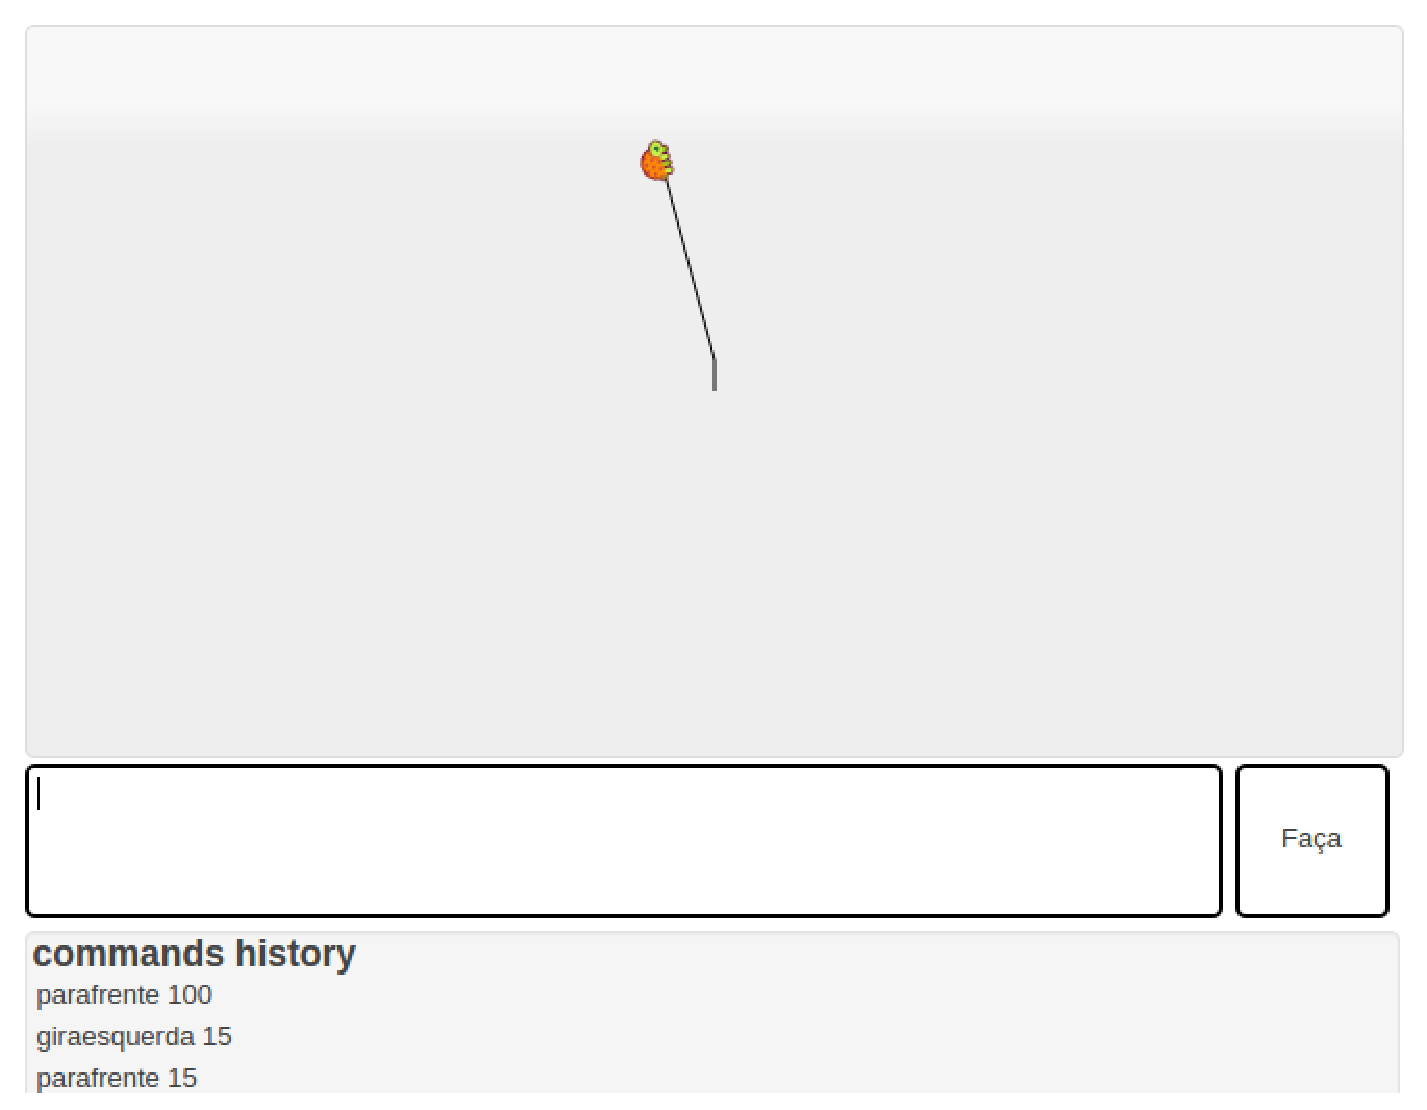
\includegraphics[scale=0.7]{figuras/ambienteLogo.eps}
			\label{img:processoGeralRevisao}
		\end{figure}

	\subsection{Planejamento da Revisão} % (fold)
	\label{sub:planejamentoRevisao}

		Esta revisão sistemática se deu entre os meses de março e junho de 2016, utilizando como fonte de busca as bases \textit{IEEE}, \textit{CAPES}, \textit{Springer} e \textit{Scopus}. A partir dos modelos de revisão sistemática apresentados por \cite{Kitchenham} e \cite{exemploRevisaoSistematica}, foi desenvolvido um protocolo de revisão, o qual possibilita, a outros pesquisadores, repetir a pesquisa.

		\subsubsection{Objetivos e questão de pesquisa}
		
		O objetivo inicial do trabalho é estudar a problemática da auto-localização na robótica, identificando diferentes soluções em diversos contextos. Afirmado isso, foi possível realizar uma pesquisa bibliográfica com o objetivo de identificar diferentes linhas de pesquisa nesta área. Após uma análise superficial de cada linha de pesquisa, foi selecionada a linha de pesquisa que adota, como solução para a auto-localização, a utilização da técnica de SLAM, o que pode ser considerado como o marco teórico do trabalho. 

		Com a identificação do marco teórico do trabalho, a definição do foco da pesquisa se torna uma tarefa menos árdua. Como o marco teórico deste trabalho se baseia nas linhas de pesquisa que buscam utilizar a técnica de SLAM para realizar navegação autônoma, esta revisão sistemática teve como objetivo identificar diferentes técnicas utilizadas atualmente para solucionar o problema de SLAM em diferentes contextos, desde contextos simplificados até contextos altamente complexos.

		A definição deste objetivo da revisão se dá pela necessidade de conhecimento amplo em relação a diferentes técnicas para solucionar o problema de SLAM. Como este trabalho buscará adaptar técnicas para um contexto simplificado, ou educacional, adicionou-se aos objetivos da revisão itens relacionados a robótica educacional e robôs simples.

		Segundo \cite{Kitchenham}, o primeiro passo para se realizar uma revisão sistemática é definir a sua questão de pesquisa. Desse modo, a partir da realização de uma pesquisa bibliográfica inicial, a questão de pesquisa foi definida como: \textit{"Como tratar o problema de SLAM no contexto de robôs simples?"}, de acordo com os objetivos da revisão, já apresentados acima.


		\subsubsection{Estratégias de pesquisa}

		A partir da definição da questão de pesquisa e dos objetivos da revisão, desenvolveu-se uma \textit{string} de busca inicial, a qual é apresentada no tópico \ref{sub:string_inicial}.

		\subsubsection{\textit{String} de busca inicial} % (fold)
		\label{sub:string_inicial}
		
			Com o objetivo de identificar pesquisas relacionadas a auto-localização utilizando mapeamento de ambientes simultaneamente, a \textit{string} de busca definida foi: \textit{auto-localization AND environment mapping}. Na tabela \ref{tab:string_inicial} são apresentados os resultados obtidos a partir desta busca.

			\begin{table}[H]
			\centering
			\caption{Resultados obtidos com a \textit{string} inicial}
			\label{tab:string_inicial}
			\begin{tabular}{|c|c|c|}
			\hline
			\rowcolor[HTML]{C0C0C0} 
			\textbf{String}                                                                                    & \multicolumn{2}{c|}{\cellcolor[HTML]{C0C0C0}\textbf{IEEE, Springer, Scopus e CAPES}}                                       \\ \hline
			                                                                                                   & \begin{tabular}[c]{@{}c@{}}Nº.\\ Artigos\end{tabular} & \begin{tabular}[c]{@{}c@{}}Nº.\\ Artigos\\ relevantes\end{tabular} \\ \hline
			\textit{\begin{tabular}[c]{@{}c@{}}Auto-localization \\ AND\\ environment \\ mapping\end{tabular}} & 36                                                    & 12                                                                 \\ \hline
			\end{tabular}
			\end{table}
		% subsection subsection_name (end)

		\subsubsection{Procedimento de seleção}

		\subsubsection{Avaliação da Qualidade}

		\subsubsection{Extração de dados}

		Entre os resultados relevantes obtidos com a busca, se encontram alguns artigos que foram classificados como artigos base para a realização da revisão sistemática, \textbf{como mostra a tabela} \ref{tab:artigos_base}. A partir destes artigos, foi possível identificar parte dos pilares que sustentam as pesquisas na área.  Com a identificação destes artigos, foi possível aplicar o conceito de \textit{quasi-gold standard}, como apresenta o tópico \ref{sub:quasi-gold}.

		\subsubsection{\textit{Quasi-gold standard}} % (fold)
		\label{sub:quasi-gold}

			Segundo \cite{quasi_goldES}, \textit{gold standard} representa o conjunto completo de estudos primários referentes a uma questão de pesquisa, com máxima precisão e sensitividade. Já o \textit{quasi-gold standard}, representa um subconjunto do \textit{gold standard}, o qual vai sendo evoluído ao longo dos ciclos de busca, com o objetivo de se aproximar do \textit{gold standard}. 

			É utilizado para definir os valores de precisão e sensitividade da busca, o que possibilita a avaliação da busca realizada, verificando a necessidade de refinamento da \textit{string}, por exemplo. \cite{quasi_goldES} define precisão e sensitividade da busca da seguinte forma:

			\begin{itemize}

				\item $precisão = \frac{ERO}{EO}$ e

				\item $sensitividade = \frac{ERO}{TER}$,
			\end{itemize}

			onde \textit{ERO} = número de estudos relevantes obtidos,
			
			\textit{EO} = número de estudos obtidos e

			\textit{TER} = número total de estudos relevantes

		
		% subsection textit_quasi_gold_standard (end)
	% subsection planejamento_da_revisão (end)

	\subsection{Condução da Revisão} % (fold)
	\label{sub:conducaoRevisao}
		
		Durante a condução da revisão, a busca efetiva dos materiais é realizada, os ciclos de busca são documentados e a \textit{string} de busca é refinada, como mostra \cite{estudoPrimarioSecundario}.
	% subsection condução_da_revisão (end)

	\subsection{Publicação dos Resultados} % (fold)
	\label{sub:publicacaoRevisao}
		
		Os resultados obtidos durante essa revisão sistemática são, além de todo o conhecimento obtido com a revisão, registrados como as técnicas utilizadas atualmente para solucionar o problema de SLAM em diferentes contextos. Com a identificação e análise destas técnicas, a possibilidade de seleção e adaptação para um contexto simplificado se torna viável. Desse modo, estão listadas, a seguir, as técnicas mais utilizadas encontradas durante a revisão.


	% subsection publicação_dos_resultados (end)

% section revisão_sistemática (end)

\section{Desenvolvimento prático} % (fold)
\label{sec:desenvolvimento_prático}

	Apresentar detalhes sobre a utilização de ferramentas, conhecimentos obtidos com a prova de conceito, problemas encontrados, soluções e etc.
% section desenvolvimento_prático (end)

\section{Ações futuras} % (fold)
\label{sec:acoes_futuras}

	Durante a segunda etapa do trabalho, pretende-se evoluir a prova de conceito apresentada durante esta primeira etapa, buscando solucionar, de maneira simplificada, o problema de SLAM. A partir dos ciclos de desenvolvimento, serão realizadas análises referentes às peculiaridades encontradas ao implementar uma técnica de auto-localização em robôs simples, assim como o impácto desta implementação em um contexto educacional.

% section section_name (end)